\documentclass[a4paper,oneside,12pt]{article}
\usepackage[utf8]{inputenc}
\usepackage{graphicx}
\usepackage{t1enc}
\usepackage[magyar]{babel}
\usepackage{hyperref}
\usepackage{pdflscape}
\usepackage{caption}
\usepackage{times}
\usepackage{listings}
\lstset{language=Java}
\usepackage{multirow}
\selectlanguage{magyar}
\frenchspacing
\linespread{1.3}
\setlength\lefthyphenmin{2} % legalább két karakter a kötőjel előtt
\setlength\righthyphenmin{2}% legalább két karakter a kötőjel után
\setlength\hyphenpenalty{0} % nem baj, ha elválasztunk a sor végén
\usepackage{fancyhdr}
\setlength{\headheight}{15.2pt}
\pagestyle{fancy}
\lhead{Fejlesztői dokumentáció}  
\rhead{Likker Ádám -- OXWQXX}


\hypersetup{
    colorlinks,
    citecolor=black,
    filecolor=black,
    linkcolor=black,
    urlcolor=blue
}



\begin{document}
\begin{titlepage}
	\pagestyle{empty}
	\begin{center}
		{\vfill \bf {\LARGE  
\includegraphics[width=90mm,keepaspectratio]{BMElogo.png} \\[90pt] Küldemény nyilvántartó rendszer \\Fejlesztői dokumentáció\\[60pt]} \Large Szoftverfejlesztés J2EE platformon\\[90pt] Likker Ádám -- OXWQXX}
	\end{center}
\end{titlepage}
\section{Célkitűzés}
Alkalmazás, mely egy futárszolgálat számára nyújt belső adminisztrációs lehetőséget
(a cég alkalmazottai használják a küldemények felvételére, számontartására, kézbesítéshez),
valamint webszolgáltatás segítségével megtekinthetők az elvállalt küldemények.
\section{Követelmények}
\subsection{Funkcionális követelmények -- használati esetek}
\begin{center}
        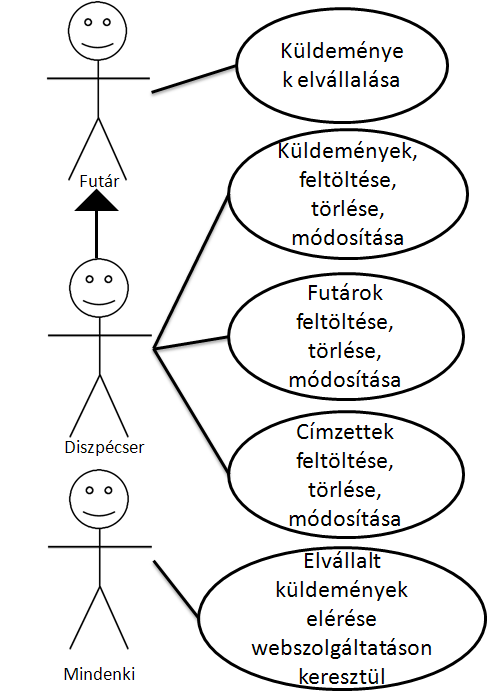
\includegraphics[width=6cm]{usecase.PNG}
	\captionof{figure}{Használati esetek}
        \label{fig:ntier}
\end{center}
\subsubsection{Szerepkörök}
Zárt rendszer, használata bejelentkezéshez kötött. Webszolgáltatást bárki elérheti.
\\\textbf{Futár} -- látja a még nem teljesített rendeléseket, elvállalja, teljesíti őket
(aki be van jelentkezve, az kerül automatikusan a teljesítéshez)
\\\textbf{Diszpécser} -- felveszi a rendeléseket, összekapcsolja a címzetteket
a küldeményekkel. Küldemények, futárok, címzettek feltöltése, törlése, módosítása

\subsection{Nem funkcionális követelmények}
Az alkalmazás legyen könnyen kezelhető, egyszerűen karbantartható. Legyen stabil (nem omlik össze, hibatűrő a bemenetekre). 
\subsubsection{Fejlesztési/futtatási környezet}
\begin{itemize}
	\item Windows vagy Linux operációs rendszer 
	\item Java 7
	\item Maven 3 build automatizációs eszköz
\end{itemize}
\section{Alkalmazás logika}
N rétegű architektúrában került implementálásra az alkalmazás, vékony klienssel, MVC (model-view-controller) tervezési
mintát szem előtt tartva.
\begin{center}
        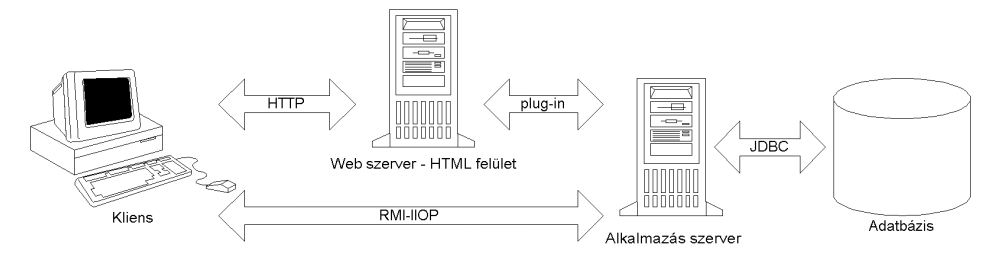
\includegraphics[width=14cm]{n-tier.PNG}
	\captionof{figure}{Az n rétegű architektúra}
        \label{fig:ntier}
\end{center}
A projekt egy fő Maven projektből áll, ami három modult fog össze:
\begin{itemize}
        \item jee-ear: Az enterprise projekt csomagolásáért felelő rész
        \item jee-ejb: Üzleti logika + beágyazott adatbázis
        \item jee-web: Megjelenítés (webes technológia)
\end{itemize}
\subsection{Csomagok}
\verb+hu.bme+\\
\verb+hu.bme.entities+
\subsection{Adatbázis}
\begin{center}
        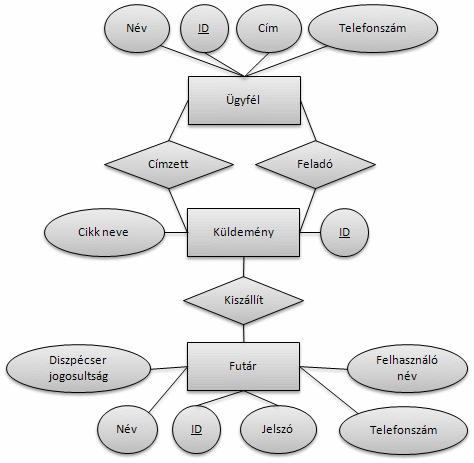
\includegraphics[width=14cm]{er.PNG}
	\captionof{figure}{Entitás relációs diagramja az alkalmazásnak}
        \label{fig:ntier}
\end{center}
Apache Derby beágyazott relációs adatbázis-kezelő rendszert használ az alkalmazás.
Az entitásokat három osztály írja le, populálásukat a \verb+StartupListener+ végzi:
\begin{itemize}
	\item \verb+Customer+ -- ügyfelek táblája
	\item \verb+Delivery+ -- küldemények táblája
	\item \verb+Runner+ -- futárok táblája
\end{itemize}
\begin{center}
        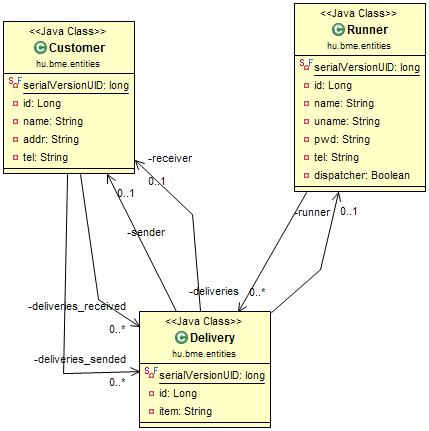
\includegraphics[width=14cm]{entities.PNG}
	\captionof{figure}{Entitások}
        \label{fig:entities}
\end{center}

\subsection{Üzleti logika}
Az üzleti logikát a \verb+SessionBean+ osztály valósítja meg.

\subsection{Webes réteg}
A webes réteg állományai, egy-egy nézetet valósítanak meg JSF technológiával
(xhtml állományok), navigációs diagram \aref{fig:nav-diag}.~ábrán: 
\begin{itemize}
\item \verb+editcustomer+ -- adott ügyfél adatainak módosítása
\item \verb+editdelivery+ -- adott küldemény adatainak módosítása
\item \verb+editrunner+ -- adott küldemény adatainak módosítása
\item \verb+failed_auth+ -- sikertelen bejelentkezéskor ide irányít át az alkalamzás
\item \verb+listcustomer+ -- ügyfelek listázása
\item \verb+listrunner+ -- futárok listázása
\item \verb+listdelivery+ -- küldemények listázása
\item \verb+loginpage+ -- bejelentkezésre szolgáló oldal
\item \verb+mainpage+ -- fő oldal, innen lehet továbbhaladni a többi nézethez
\item \verb+newcustomer+ -- új ügyfél felvétele
\item \verb+newdelivery+ -- új küldemény felvétele
\item \verb+newrunner+ -- új futár felvétele
\item \verb+succ_auth+ -- sikeres bejelentkezéskor megjelenő oldal
\end{itemize}
%
Az egyes nézeteket az alábbi backing beanek működtetik:
\begin{itemize}
\item \verb+CustomerMBean+ -- Ügyfelek adatainak módosítása
\item \verb+DeliveryMBean+ -- Küldemények adatainak módosítása
\item \verb+LoginBean+ -- Bejelentkezés kezelése 
\item \verb+MainMBean+  -- Backing bean listázása, új entitások létrehozása
\item \verb+RunnerMBean+ -- Futárok adatainak módosítása
\end{itemize}
\begin{center}
        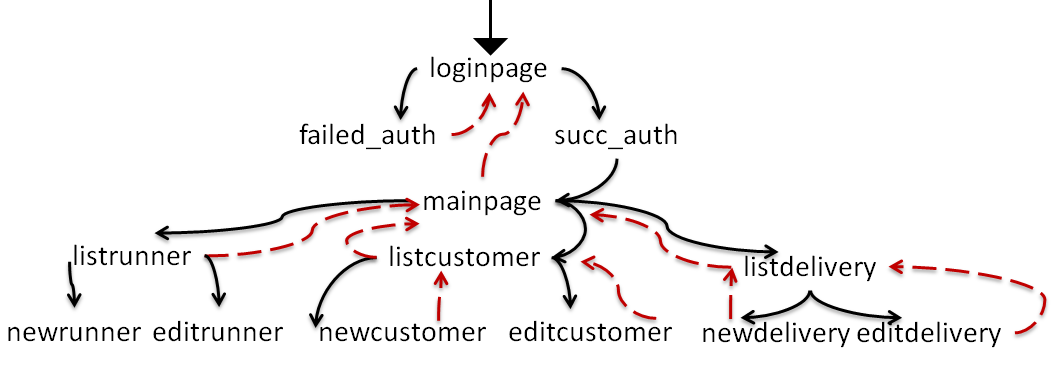
\includegraphics[width=14cm]{nav_diag.png}
        \captionof{figure}{Navigációs diagram}
        \label{fig:nav-diag}
\end{center}
\begin{center}
        \includegraphics[width=14cm]{webclass.png}
        \captionof{figure}{Backing beanek}
        \label{fig:webclass}
\end{center}
\subsection{Webszolgáltatás }
\verb+ListAccDeliveryService+ -- kilistázza azon küldeményeket, amikhez tartozik futár
(azaz elvállalta valaki a küldemény teljesítését)
\end{document}
